
%% APPENDICES

\begin{figure}
	\begin{center}
		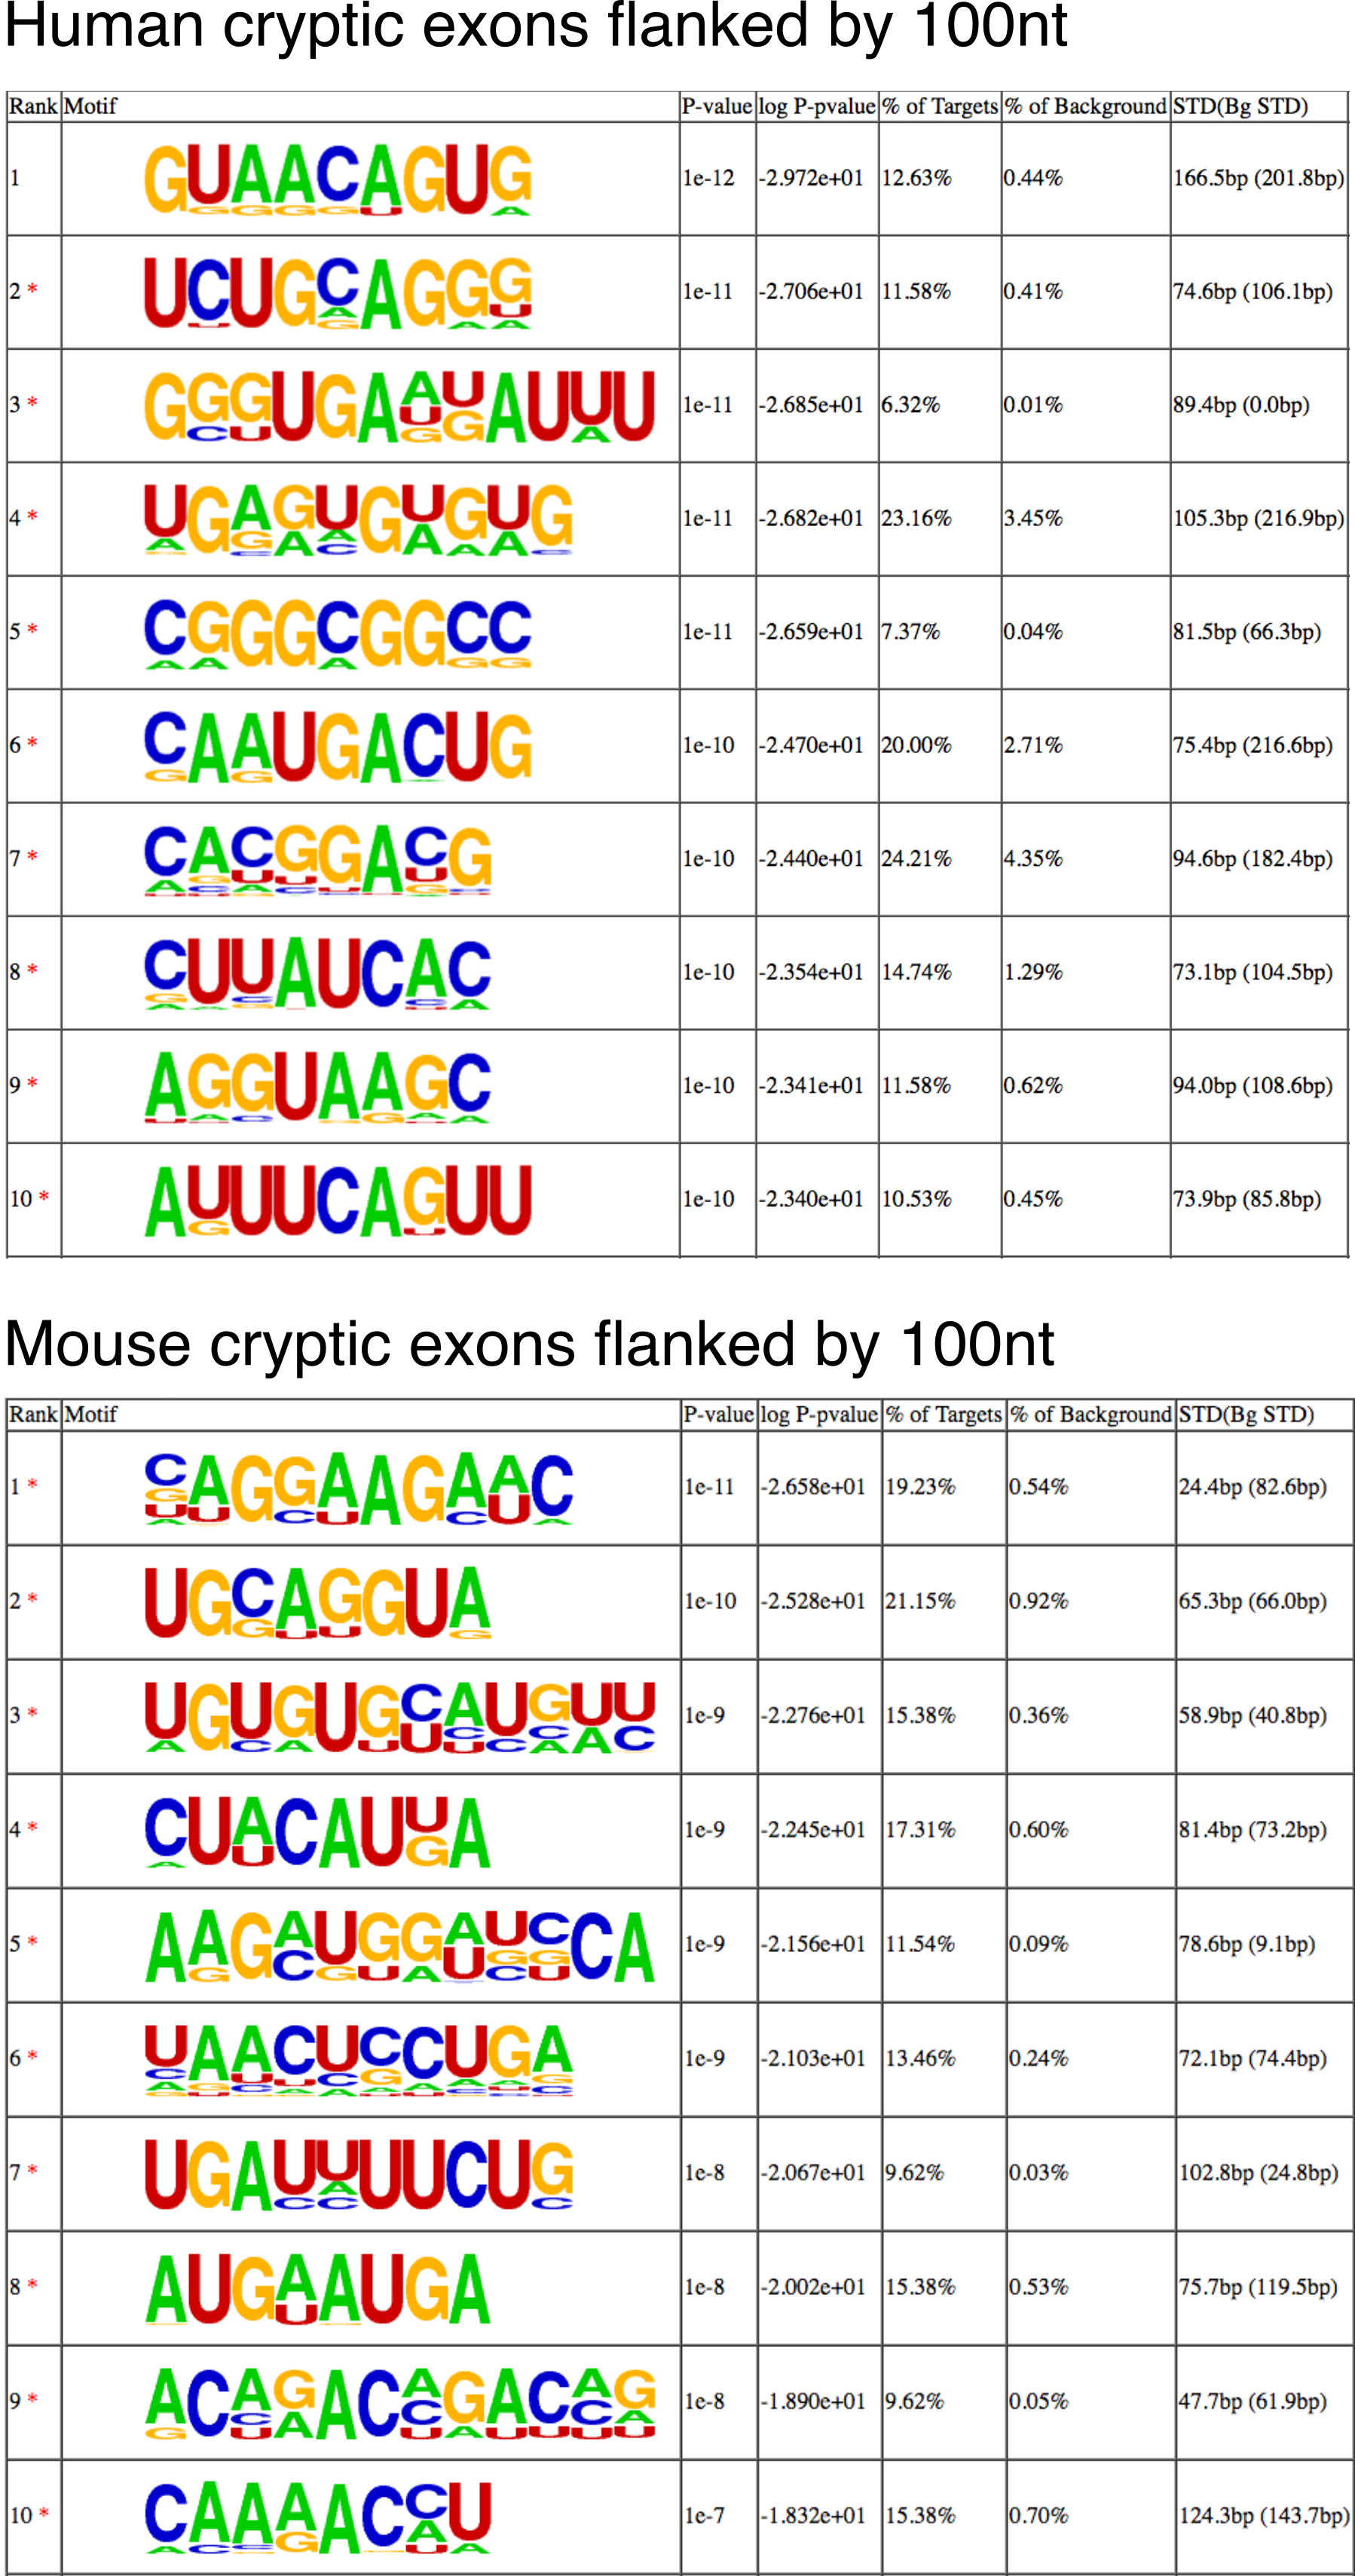
\includegraphics[width=10cm]{Appendices/Figure_S4_HOMER.png}
	\end{center}
	\caption{Motifs found by \textit{HOMER}}
\end{figure}


%\pagenumbering{gobble}
\addtolength{\abovecaptionskip}{-25mm}
% mouse table
\newgeometry{left=3cm,bottom=0.8cm}
\begin{landscape}
	
% Table generated by Excel2LaTeX from sheet 'ST1_mouse_summary_table.tsv'
%\begin{table}[htbp]
% Table generated by Excel2LaTeX from sheet 'ST1_mouse_summary_table.tsv'
\begin{table}[htbp]
	\centering
	2. All mouse cryptic exons discovered by \textit{CryptEx}
	\tiny
	\resizebox{\columnwidth}{!}{
	%\caption{All mouse cryptic exons discovered in chapter 3}
	\begin{tabular}{|l|c|l|l|l|l|c|c|c|l|l|l|l|l|l|}
		\hline
		\multicolumn{15}{|c|}{\cellcolor[HTML]{EFEFEF}{}} \\ \hline
		gene & Ensembl ID & exon ID & chr & exon start & exon end &+/-&5'$\Delta$PSI&3'$\Delta$PSI&classification&observed in&EScell $log_2$FC&brain $log_2$FC&\textit{phyloP}&prediction\\
		\hline
		\textit{Abr} & ENSMUSG00000017631 & E026i1 & chr11 & 76468524 & 76468676 & -     & 0.09  & 0.00  & 5' extension & EScell;brain & -1.75 & -0.59 & 0.77  & PTC/frame shifted \\ \hline
		\textit{Pnpla6} & ENSMUSG00000004565 & E016i1 & chr8  & 3524947 & 3525140 & +     & 0.29  & 0.00  & 5' extension & brain & -1.56 & -0.47 & 0.08  & PTC/frame shifted \\ \hline
		\textit{Lrrc49} & ENSMUSG00000047766 & E017i3 & chr9  & 60637648 & 60637695 & -     & 0.06  & 0.00  & 5' extension & brain & -1.19 & -0.25 & 0.17  & PTC/frame shifted \\ \hline
		\textit{Ccdc149} & ENSMUSG00000045790 & E009i3 & chr5  & 52434250 & 52434424 & -     & 0.16  & 0.00  & 5' extension & brain & .     & -0.28 & 0.06  & PTC/frame conserved \\ \hline
		\textit{Ak5} & ENSMUSG00000039058 & E014i6 & chr3  & 152643869 & 152643915 & -     & 0.16  & 0.00  & 5' extension & brain & .     & -0.53 & 0.17  & PTC/frame shifted \\ \hline
		\textit{Kctd10} & ENSMUSG00000001098 & E017i2 & chr5  & 114376677 & 114376866 & -     & 0.07  & 0.01  & 5' extension & brain & .     & .     & 0.02  & PTC/frame shifted \\ \hline
		\textit{Tmem14a} & ENSMUSG00000025933 & E005i1 & chr1  & 21229121 & 21229173 & +     & 0.37  & 0.00  & 5' extension & brain & -1.02 & -0.60 & -0.08 & PTC/frame conserved \\ \hline
		\textit{Apod} & ENSMUSG00000022548 & E006i1 & chr16 & 31298051 & 31298471 & -     & 0.04  & 0.08  & 3' extension & brain & .     & 0.74  & 0.09  & PTC/frame shifted \\ \hline
		\textit{Erbb2ip} & ENSMUSG00000021709 & E026i1 & chr13 & 103862527 & 103862588 & -     & 0.00  & 0.25  & 3' extension & brain & .     & 0.62  & -0.05 & PTC/frame shifted \\ \hline
		\textit{Trim8} & ENSMUSG00000025034 & E001i2 & chr19 & 46506869 & 46506928 & +     & 0.00  & 0.10  & 3' extension & Ling;brain & .     & .     & -0.23 & PTC/frame shifted \\ \hline
		\textit{Usp15} & ENSMUSG00000099088 & E015i3 & chr10 & 123150961 & 123151125 & -     & 0.00  & 0.32  & 3' extension & Ling;brain & .     & .     & 0.15  & PTC/frame conserved \\ \hline
		\textit{Fam135a} & ENSMUSG00000026153 & E008i1 & chr1  & 24022506 & 24022670 & -     & 0.00  & 0.25  & 3' extension & brain & .     & .     & 0.00  & PTC/frame shifted \\ \hline
		\textit{Rasal1} & ENSMUSG00000029602 & E007i1 & chr5  & 120653508 & 120653879 & +     & 0.03  & 0.16  & 3' extension & brain & .     & .     & -0.23 & PTC/frame conserved \\ \hline
		\textit{Brms1l} & ENSMUSG00000012076 & E008i1 & chr12 & 55864624 & 55865091 & +     & 0.04  & 0.23  & 3' extension & brain & -0.81 & .     & 0.14  & PTC/frame conserved \\ \hline
		\textit{Cacna1b} & ENSMUSG00000004113 & E050i1 & chr2  & 24691959 & 24692366 & -     & 0.00  & 0.39  & 3' extension & brain & .     & -0.58 & 0.21  & PTC/frame shifted \\ \hline
		\textit{Nt5c3b} & ENSMUSG00000017176 & E010i1 & chr11 & 100433637 & 100433684 & -     & 0.00  & 0.07  & 3' extension & brain & -1.15 & -0.50 & 0.12  & PTC/frame conserved \\ \hline
		\textit{Spcs2} & ENSMUSG00000035227 & E004i1 & chr7  & 99856412 & 99856514 & -     & 0.01  & 0.29  & 3' extension & Ling;EScell;brain & .     & 0.34  & 0.40  & PTC/frame shifted \\ \hline
		\textit{Ccdc88a} & ENSMUSG00000032740 & E004i8 & chr11 & 29421354 & 29421401 & +     & 0.00  & 0.27  & 3' extension & brain & -1.63 & .     & -0.04 & PTC/frame conserved \\ \hline
		\textit{Adap1} & ENSMUSG00000056413 & E014i3 & chr5  & 139302108 & 139302166 & -     & 0.00  & 0.36  & 3' extension & brain & .     & -0.47 & 0.08  & PTC/frame shifted \\ \hline
		\textit{Ap3b2} & ENSMUSG00000062444 & E031i2 & chr7  & 81490178 & 81490277 & -     & 0.04  & 0.10  & 3' extension & brain & 0.50  & -0.28 & 0.18  & PTC/frame shifted \\ \hline
		\textit{Fam73a} & ENSMUSG00000054942 & E015i2 & chr3  & 152292556 & 152292657 & -     & 0.02  & 0.09  & 3' extension & Ling;brain & -1.39 & -0.63 & -0.04 & PTC/frame shifted \\ \hline
		\textit{Ptprn2} & ENSMUSG00000056553 & E019i11 & chr12 & 117154249 & 117154298 & +     & 0.00  & 0.13  & 3' extension & brain & .     & -1.01 & 0.24  & PTC/frame shifted \\ \hline
		\textit{Dlg2} & ENSMUSG00000052572 & E004i17 & chr7  & 91543136 & 91543191 & +     & 0.00  & 0.23  & 3' extension & brain & .     & -0.71 & 1.67  & PTC/frame shifted \\ \hline
		\textit{Cd200} & ENSMUSG00000022661 & E003i1 & chr16 & 45389970 & 45390184 & -     & 0.04  & 0.06  & 3' extension & brain & .     & .     & -0.13 & Not in CDS \\ \hline
		\textit{Dock4} & ENSMUSG00000035954 & E049i1 & chr12 & 40835769 & 40835912 & +     & 0.09  & 0.20  & Cassette & brain & .     & -0.68 & 0.53  & PTC/frame shifted \\ \hline
		\textit{C4b} & ENSMUSG00000073418 & E032i1 & chr17 & 34739389 & 34739500 & -     & 0.06  & 0.30  & Cassette & brain & .     & .     & 0.00  & PTC/frame shifted \\ \hline
		\textit{Camk1g} & ENSMUSG00000016179 & E017i2 & chr1  & 193368866 & 193368952 & -     & 0.70  & 0.47  & Cassette & brain & .     & .     & -0.06 & Not in CDS  \\ \hline
		\textit{Reep3} & ENSMUSG00000019873 & E001i1 & chr10 & 67014087 & 67014164 & -     & 0.67  & 0.39  & Cassette & brain & .     & 0.44  & -0.01 & PTC/frame shifted \\ \hline
		\textit{Drosha} & ENSMUSG00000022191 & E009i1 & chr15 & 12833221 & 12833389 & +     & 0.10  & 0.15  & Cassette & brain & .     & .     & -0.06 & PTC/frame conserved \\ \hline
		\textit{Synj2bp} & ENSMUSG00000021139 & E036i2 & chr12 & 81509671 & 81510249 & -     & 0.41  & 0.07  & Cassette & brain & .     & .     & 0.11  & PTC/frame shifted \\ \hline
		\textit{Adnp2} & ENSMUSG00000053950 & E002i1 & chr18 & 80138152 & 80138304 & -     & 0.57  & 0.50  & Cassette & Ling;EScell;brain & 0.33  & 0.25  & 0.03  & PTC/frame shifted \\ \hline
		\textit{Adipor2} & ENSMUSG00000030168 & E010i2 & chr6  & 119369859 & 119369918 & -     & 0.30  & 0.44  & Cassette & Ling;brain & -1.06 & .     & 0.07  & PTC/frame shifted \\ \hline
		\textit{Cdh22} & ENSMUSG00000053166 & E013i2 & chr2  & 165183238 & 165183371 & -     & 0.40  & 0.67  & Cassette & brain & .     & -0.35 & 0.13  & Not in CDS \\ \hline
		\textit{Ermn} & ENSMUSG00000026830 & E001i1 & chr2  & 58049485 & 58049561 & -     & 0.16  & 0.16  & Cassette & brain & .     & .     & 0.06  & PTC/frame shifted \\ \hline
		\textit{Ift81} & ENSMUSG00000029469 & E003i1 & chr5  & 122556905 & 122556991 & -     & 0.19  & 0.08  & Cassette & Ling;brain & .     & .     & 0.08  & benign/frame shifted \\ \hline
		\textit{Vps13d} & ENSMUSG00000020220 & E043i1 & chr4  & 145099351 & 145099463 & -     & 0.60  & 0.20  & Cassette & brain & .     & -0.81 & 0.23  & PTC/frame shifted \\ \hline
		\textit{Ube2d1} & ENSMUSG00000019927 & E010i1 & chr10 & 71263584 & 71263717 & -     & 0.15  & 0.36  & Cassette & EScell;brain & .     & 0.35  & 0.04  & PTC/frame shifted \\ \hline
		\textit{Hgsnat} & ENSMUSG00000037260 & E001i1 & chr8  & 25945947 & 25945999 & -     & 0.28  & 0.15  & Cassette & Ling;brain & -0.59 & .     & 0.20  & PTC/frame conserved \\ \hline
		\textit{Elmod1} & ENSMUSG00000041986 & E003i2 & chr9  & 53923941 & 53923995 & -     & 0.27  & 0.19  & Cassette & brain & .     & .     & 0.97  & benign/frame conserved \\ \hline
		\textit{Mkx} & ENSMUSG00000061013 & E007i7 & chr18 & 6986138 & 6986235 & -     & 0.24  & 0.50  & Cassette & brain & .     & .     & -0.08 & PTC/frame shifted \\ \hline
		\textit{Hace1} & ENSMUSG00000038822 & E013i1 & chr10 & 45639722 & 45639803 & +     & 0.06  & 0.20  & Cassette & Ling;brain & .     & -0.38 & 0.10  & benign/frame conserved \\ \hline
		\textit{Fxyd2} & ENSMUSG00000059412 & E003i1 & chr9  & 45408987 & 45409173 & +     & 0.42  & 0.18  & Cassette & brain & -1.89 & .     & -0.25 & PTC/frame shifted \\ \hline
		\textit{Thoc7} & ENSMUSG00000053453 & E007i1 & chr14 & 13957061 & 13957631 & -     & 0.21  & -0.10 & 5' extension & EScell & -0.74 & .     & 0.04  & PTC/frame shifted \\ \hline
		\textit{Nme6} & ENSMUSG00000032478 & E020i1 & chr9  & 109837872 & 109838225 & +     & 0.40  & 0.00  & 5' extension & Ling;EScell & -0.84 & .     & 0.21  & PTC/frame conserved \\ \hline
		\textit{Wtip} & ENSMUSG00000036459 & E001i1 & chr7  & 34111074 & 34111099 & -     & 0.13  & 0.00  & 5' extension & EScell & -0.46 & .     & 0.26  & PTC/frame shifted \\ \hline
		\textit{Gsta4} & ENSMUSG00000032348 & E005i2 & chr9  & 78207196 & 78207382 & +     & 0.02  & 0.07  & 3' extension & Ling;EScell & -0.45 & .     & 0.11  & PTC/frame shifted \\ \hline
		\textit{Slc7a6} & ENSMUSG00000031904 & E001i1 & chr8  & 106169186 & 106169256 & +     & 0.00  & 0.12  & 3' extension & EScell & .     & -0.23 & -0.25 & Not in CDS \\ \hline
		\textit{Flnb} & ENSMUSG00000025278 & E040i1 & chr14 & 7935368 & 7935630 & +     & 0.09  & 0.43  & Cassette & Ling;EScell;brain & -1.34 & .     & -0.12 & PTC/frame shifted \\ \hline
		\textit{B4galnt3} & ENSMUSG00000041372 & E002i1 & chr6  & 120204263 & 120204465 & -     & 0.07  & 0.10  & Cassette & EScell & .     & .     & -0.15 & PTC/frame shifted \\ \hline
		\textit{Psma2} & ENSMUSG00000015671 & E005i1 & chr13 & 14620930 & 14621038 & +     & 0.06  & 0.13  & Cassette & EScell & .     & .     & 0.19  & PTC/frame conserved \\ \hline
		\textit{Abr} & ENSMUSG00000017631 & E024i1 & chr11 & 76464580 & 76464758 & -     & 0.18  & 0.07  & Cassette & EScell;brain & -1.75 & -0.59 & -0.25 & PTC/frame shifted \\ \hline
		\textit{Wasf3} & ENSMUSG00000029636 & E009i1 & chr5  & 146469766 & 146469912 & +     & 0.10  & 0.22  & Cassette & EScell & .     & .     & -0.02 & benign/frame conserved \\ \hline
	\end{tabular}%
	}
\end{table}%

\clearpage

%% Table generated by Excel2LaTeX from sheet 'ST2_human_summary_table.tsv'
\begin{table}
	\centering
	3. All human cryptic exons discovered by \textit{CryptEx}
	\tiny
	\resizebox{\columnwidth}{!}{ 
%	\fontsize{5}{6}
	\begin{tabular}{|l|c|l|l|l|l|c|c|c|l|l|l|l|l|l|l|l|}
		\hline
%		\multicolumn{17}{Human cryptic exons} \\ 
		\multicolumn{17}{|c|}{\cellcolor[HTML]{EFEFEF}{} } \\ 
		\hline
		gene&Ensembl ID&exon ID&chr&exon start&exon end&+/-& 5'$\Delta$PSI&3'$\Delta$PSI& classification& observed in &mRNA FC&total FC&\textit{phyloP}&prediction&\textit{maxEnt} 5'&\textit{maxEnt} 3'\\ \hline 
		\textit{PHF12} & ENSG00000109118 & E028i1 & chr17 & 28914903 & 28915475 & -     & 0.14  & 0.00  & 5' extension & mRNA;total & 0.23  & . & 0.448493 & PTC/frame conserved & . &  9.93 \\ \hline
		\textit{ZFPM2} & ENSG00000169946 & E016i1 & chr8  & 105419822 & 105419906 & +     & 0.35  & 0.00  & 5' extension & mRNA  & . & . & -0.131815 & PTC/frame conserved & . &  11.28 \\ \hline
		\textit{ACBD3} & ENSG00000182827 & E004i1 & chr1  & 226156701 & 226156780 & -     & 0.12  & 0.00  & 5' extension & mRNA  & -0.31 & . & 0.22671 & PTC/frame shifted & . &  9.63 \\ \hline
		\textit{RPS6KA3} & ENSG00000177189 & E031i2 & chrX  & 20241592 & 20241686 & -     & 0.18  & 0.01  & 5' extension & mRNA  & -0.42 & . & 2.38738 & PTC/frame shifted & . &  8.09 \\ \hline
		\textit{CPED1} & ENSG00000106034 & E034i7 & chr7  & 121194471 & 121194593 & +     & 0.07  & 0.01  & 5' extension & mRNA  & . & . & 0.398074 & PTC/frame shifted & . &  9.56 \\ \hline
		\textit{HUWE1} & ENSG00000086758 & E033i1 & chrX  & 53551990 & 53552074 & -     & 0.09  & 0.05  & 5' extension & mRNA  & -0.56 & . & 0.114241 & PTC/frame shifted & . &  6.87 \\ \hline
		\textit{DYNC2LI1} & ENSG00000138036 & E006i1 & chr2  & 43774402 & 43774936 & +     & 0.08  & 0.04  & 5' extension & mRNA  & -0.63 & . & -0.228969 & PTC/frame shifted & . &  2.09 \\ \hline
		\textit{ZMYND8} & ENSG00000101040 & E019i2 & chr20 & 47254235 & 47254424 & -     & 0.07  & 0.03  & 5' extension & mRNA  & -0.36 & . & 0.101961 & PTC/frame shifted & . &  3.77 \\ \hline
		\textit{HEPH} & ENSG00000089472 & E030i1 & chrX  & 66257344 & 66257516 & +     & 0.12  & 0.00  & 5' extension & mRNA  & -0.58 & -0.34 & 0.245606 & PTC/frame shifted & . &  14.19 \\ \hline
		\textit{BTNL9} & ENSG00000165810 & E031i1 & chr5  & 181059149 & 181059215 & +     & 0.09  & 0.00  & 5' extension & mRNA  & . & . & -0.101275 & PTC/frame shifted & . &  -0.66 \\ \hline
		\textit{PAPSS1} & ENSG00000138801 & E008i1 & chr4  & 107654948 & 107655036 & -     & 0.08  & 0.00  & 5' extension & mRNA;total & -0.87 & . & 0.746813 & PTC/frame conserved & . &  10.84 \\ \hline
		\textit{CLASP1} & ENSG00000074054 & E049i1 & chr2  & 121471187 & 121471274 & -     & 0.16  & 0.00  & 5' extension & mRNA  & -0.19 & . & -0.0460715 & PTC/frame shifted & . &  4.56 \\ \hline
		\textit{IST1} & ENSG00000224470 & E053i1 & chr16 & 71922108 & 71922437 & +     & 0.12  & 0.01  & 5' extension & mRNA  & . & . & 0.177172 & PTC/frame shifted & . &  13.96 \\ \hline
		\textit{UBR4} & ENSG00000272084& E084i1 & chr1  & 19145598 & 19145708 & -     & 0.05  & 0.00  & 5' extension & mRNA  & . & . & 0.710974 & PTC/frame shifted & . &  7.28 \\ \hline
		\textit{ANKRD27} & ENSG00000105186 & E019i1 & chr19 & 32630070 & 32630151 & -     & 0.15  & 0.01  & 5' extension & mRNA  & -0.37 & -0.24 & -0.103821 & PTC/frame shifted & . &  12.52 \\ \hline
		\textit{CCDC77} & ENSG00000120647 & E020i1 & chr12 & 422421 & 422891 & +     & 0.07  & 0.01  & 5' extension & mRNA  & -0.84 & . & -0.0231545 & PTC/frame shifted & . &  3.79 \\ \hline
		\textit{LRPPRC} & ENSG00000138095 & E024i1 & chr2  & 43942675 & 43942815 & -     & 0.06  & 0.00  & 5' extension & mRNA  & -1.01 & . & 0.14133 & PTC/frame shifted & . &  3.85 \\ \hline
		\textit{ADGRV1} & ENSG00000164199 & E085i1 & chr5  & 90803514 & 90803596 & +     & 0.07  & 0.00  & 5' extension & mRNA  & -0.47 & 0.32  & -0.185377 & PTC/frame shifted & . &  9.14 \\ \hline
		\textit{ASNSP1} & ENSG00000248498 & E006i1 & chr8  & 46595259 & 46595315 & -     & 0.13  & 0.00  & 5' extension & mRNA  & . & . & 1.14798 & Not in CDS     & . &  8.29 \\ \hline
		\textit{SMAD2} & ENSG00000175387 & E010i1 & chr18 & 47868051 & 47868103 & -     & 0.08  & 0.02  & 5' extension & mRNA  & -0.39 & . & 0.289826 & PTC/frame shifted & . &  9.95 \\ \hline
		\textit{ZNHIT6} & ENSG00000117174 & E003i1 & chr1  & 85662210 & 85662278 & -     & 0.08  & 0.04  & 5' extension & mRNA  & -0.80 & . & 0.0230322 & PTC/frame conserved & . &  5.75 \\ \hline
		\textit{NLRP1} & ENSG00000091592 & E045i1 & chr17 & 5585499 & 5585635 & -     & 0.15  & 0.00  & 5' extension & mRNA  & . & . & -0.1356 & Not in CDS     & . &  5.48 \\ \hline
		\textit{CEP290} & ENSG00000198707 & E024i1 & chr12 & 88086709 & 88086789 & -     & 0.13  & 0.00  & 5' extension & mRNA  & -1.15 & . & 0.157693 & PTC/frame shifted & . &  7.83 \\ \hline
		\textit{METTL8} & ENSG00000123600 & E037i1 & chr2  & 171433562 & 171433649 & -     & 0.50  & 0.00  & 5' extension & mRNA  & . & . & 0.223589 & Not in CDS     & . &  11.06 \\ \hline
		\textit{MPDZ} & ENSG00000107186 & E015i1 & chr9  & 13110935 & 13111024 & -     & 0.35  & 0.00  & 5' extension & mRNA  & -0.57 & . & 0.11092 & PTC/frame shifted & . &  10.52 \\ \hline
		\textit{ERBB2IP} & ENSG00000112851 & E013i2 & chr5  & 65997127 & 65997228 & +     & 0.06  & 0.04  & 5' extension & mRNA  & -0.39 & . & 0.211071 & PTC/frame shifted & . &  9.62 \\ \hline
		\textit{PRPF40A} & ENSG00000196504 & E001i1 & chr2  & 152657053 & 152657141 & -     & 0.04  & 0.05  & 3' extension & mRNA  & -0.77 & . & -0.0653744 & PTC/frame shifted & -0.49 & . \\ \hline
		\textit{UPF2} & ENSG00000151461 & E002i1 & chr10 & 11926921 & 11927006 & -     & 0.00  & 0.16  & 3' extension & Ling;mRNA & . & . & 0.00227976 & PTC/frame shifted & 9.85  & . \\ \hline
		\textit{RRP1} & ENSG00000160214 & E008i1 & chr21 & 43791522 & 43792578 & +     & 0.02  & 0.08  & 3' extension & mRNA  & 0.82  & . & -0.184698 & PTC/frame shifted & 6.51  & . \\ \hline
		\textit{LRP8} & ENSG00000157193 & E033i1 & chr1  & 53274090 & 53274694 & -     & 0.00  & 0.27  & 3' extension & mRNA;total & . & . & 1.77583 & PTC/frame conserved & 2.70  & . \\ \hline
		\textit{PKP4} & ENSG00000144283 & E020i1 & chr2  & 158588958 & 158588987 & +     & 0.00  & 0.17  & 3' extension & mRNA  & -0.31 & . & 0.0933565 & PTC/frame shifted & 3.91  & . \\ \hline
		\textit{DDX52} & ENSG00000278053 & E022i1 & chr17 & 37629848 & 37629963 & -     & 0.01  & 0.08  & 3' extension & mRNA;total & -0.39 & -0.30 & 0.981172 & PTC/frame conserved & 7.96  & . \\ \hline
		\textit{SETD5} & ENSG00000168137 & E065i1 & chr3  & 9468576 & 9468615 & +     & 0.00  & 0.13  & 3' extension & Ling;mRNA;total & -0.24 & . & 2.57544 & PTC/frame conserved & 7.36  & . \\ \hline
		\textit{KDELC2} & ENSG00000178202 & E018i2 & chr11 & 108497751 & 108498085 & -     & 0.00  & 0.19  & 3' extension & Ling;mRNA & -0.78 & . & -0.0860609 & PTC/frame conserved & 8.95  & . \\ \hline
		\textit{GPT2} & ENSG00000166123 & E009i1 & chr16 & 46900812 & 46900883 & +     & 0.00  & 0.16  & 3' extension & mRNA  & -0.98 & -0.72 & 1.01736 & PTC/frame shifted & 3.30  & . \\ \hline
		\textit{GSE1} & ENSG00000131149 & E007i1 & chr16 & 85650416 & 85650709 & +     & 0.04  & 0.06  & 3' extension & mRNA  & 0.29  & . & -0.525771 & PTC/frame shifted & 5.99  & . \\ \hline
		\textit{MBOAT2} & ENSG00000143797 & E029i2 & chr2  & 8986052 & 8986136 & -     & 0.00  & 0.25  & 3' extension & mRNA  & -0.66 & . & -0.0138646 & PTC/frame shifted & 8.34  & . \\ \hline
		\textit{DNAAF5} & ENSG00000164818 & E024i1 & chr7  & 783225 & 783309 & +     & 0.00  & 0.05  & 3' extension & mRNA  & 0.49  & -0.37 & -0.238231 & PTC/frame shifted & 9.25  & . \\ \hline
		\textit{CLASP1} & ENSG00000074054 & E012i1 & chr2  & 121387587 & 121387655 & -     & 0.04  & 0.07  & 3' extension & mRNA  & -0.19 & . & -0.0066914 & PTC/frame conserved & 2.72  & . \\ \hline
		\textit{ZFP91} & ENSG00000255073 & E012i1 & chr11 & 58616974 & 58617182 & +     & 0.04  & 0.05  & 3' extension & mRNA  & . & . & -0.213922 & PTC/frame shifted & 6.97  & . \\ \hline
		\textit{FAM178B} & ENSG00000273634 & E017i1 & chr2  & 96923867 & 96924228 & -     & 0.00  & 0.30  & 3' extension & mRNA  & . & . & -0.351309 & PTC/frame shifted & 3.14  & . \\  \hline
		\textit{ANAPC1} & ENSG00000153107 & E020i1 & chr2  & 111799529 & 111799699 & -     & 0.00  & 0.12  & 3' extension & mRNA  & -0.90 & . & 0.0276639 & PTC/frame conserved & 5.28  & . \\ \hline
		\textit{CERK} & ENSG00000100422 & E005i1 & chr22 & 46691869 & 46692022 & -     & 0.03  & 0.14  & 3' extension & mRNA  & . & . & -0.579144 & PTC/frame shifted & 9.22  & . \\ \hline
		\textit{ARHGAP11B} & ENSG00000187951 & E033i1 & chr15 & 30755981 & 30756067 & +     & 0.00  & 0.11  & 3' extension & mRNA  & . & . & -0.13533 & Not in CDS     & 10.77 & . \\ \hline
		\textit{GOLGA8A} & ENSG00000175265 & E037i1 & chr15 & 34436658 & 34436837 & -     & 0.00  & 0.10  & 3' extension & mRNA  & -0.58 & . & -0.147737 & Not in CDS     & 8.72  & . \\ \hline
		\textit{TGFBRAP1} & ENSG00000135966 & E014i2 & chr2  & 105307479 & 105307570 & -     & 0.00  & 0.19  & 3' extension & mRNA  & . & . & 0.807447 & PTC/frame shifted & 4.75  & . \\ \hline
		\textit{CAMK2G} & ENSG00000148660 & E039i1 & chr10 & 73873200 & 73873283 & -     & 0.00  & 0.21  & 3' extension & mRNA  & . & . & 0.336877 & PTC/frame shifted & 6.32  & . \\ \hline
	\end{tabular}
	}
\end{table}	
\begin{table}
	\centering
	3. All human cryptic exons discovered by \textit{CryptEx} (continued)
	\tiny
	\resizebox{\columnwidth}{!}{ 
	\begin{tabular}{|l|c|l|l|l|l|c|c|c|l|l|l|l|l|l|l|l|}
		\hline
		\multicolumn{17}{|c|}{\cellcolor[HTML]{EFEFEF}{ } } \\ 
		\hline
		gene&Ensembl ID&exon ID&chr&exon start&exon end&+/-& 5'$\Delta$PSI&3'$\Delta$PSI& classification& observed in &mRNA FC&total FC&\textit{phyloP}&prediction&\textit{maxEnt} 5'&\textit{maxEnt} 3'\\ \hline 
		\textit{DCAF17} & ENSG00000115827 & E008i1 & chr2  & 171441954 & 171442195 & +     & 0.04  & 0.07  & 3' extension & mRNA  & -0.50 & . & 0.207598 & PTC/frame conserved & 5.13  & . \\ \hline
		\textit{RP1-179N16.6} & ENSG00000246982 & E002i2 & chr6  & 36160683 & 36160784 & -     & 0.02  & 0.13  & 3' extension & mRNA  & . & . & 0.161445 & Not in CDS     & 9.16  & . \\ \hline
		\textit{RNFT2} & ENSG00000135119 & E016i2 & chr12 & 116790033 & 116790087 & +     & 0.00  & 0.15  & 3' extension & Ling;mRNA & . & . & 0.118938 & PTC/frame shifted & 7.03  & . \\ \hline
		\textit{SH2B3} & ENSG00000111252 & E005i1 & chr12 & 111446092 & 111446216 & +     & 0.00  & 0.11  & 3' extension & mRNA  & . & -0.52 & -0.401417 & PTC/frame shifted & 5.85  & . \\ \hline
		\textit{SENP7} & ENSG00000138468 & E020i1 & chr3  & 101349160 & 101349188 & -     & 0.00  & 0.05  & 3' extension & mRNA  & -1.11 & . & 0.116452 & PTC/frame shifted & 6.06  & . \\ \hline
		\textit{GOLGB1} & ENSG00000173230 & E013i1 & chr3  & 121682916 & 121682980 & -     & 0.03  & 0.08  & 3' extension & mRNA  & -0.40 & 0.26  & 0.918212 & PTC/frame conserved & 9.35  & . \\ \hline
		\textit{AGRN} & ENSG00000242590 & E015i1 & chr1  & 1044440 & 1045080 & +     & 0.46  & 0.63  & Cassette & Ling;mRNA;total & . & . & -0.913282 & PTC/frame shifted & 5.78  &  4.71 \\ \hline
\textit{CEP72} & ENSG00000112877 & E012i1 & chr5  & 648049 & 648223 & +     & 0.69  & 0.70  & Cassette & Ling;mRNA;total & . & -0.30 & -0.102364 & PTC/frame shifted & 9.81  &  -7.11 \\ \hline
\textit{RAP1GAP} & ENSG00000076864 & E010i1 & chr1  & 21598718 & 21598820 & -     & 0.27  & 0.34  & Cassette & mRNA  & . & -0.39 & -0.293165 & PTC/frame shifted & 6.51  &  7.06 \\ \hline
\textit{PFKP} & ENSG00000067057 & E010i1 & chr10 & 3099556 & 3099819 & +     & 0.29  & 0.19  & Cassette & Ling;mRNA;total & . & . & -0.0943177 & PTC/frame shifted & 4.88  &  2.02 \\ \hline
\textit{PKN1} & ENSG00000123143 & E016i2 & chr19 & 14450087 & 14450214 & +     & 0.22  & 0.10  & Cassette & Ling;mRNA & . & -0.49 & 0.0079453 & PTC/frame shifted & 4.88  &  6.94 \\ \hline
\textit{FAM114A2} & ENSG00000055147 & E040i1 & chr5  & 154037367 & 154037457 & -     & 0.27  & 0.23  & Cassette & Ling;mRNA;total & . & . & 0.205094 & Not in CDS & 8.11  &  11.04 \\ \hline
\textit{HDGFRP2} & ENSG00000167674 & E015i1 & chr19 & 4492012 & 4492152 & +     & 0.15  & 0.10  & Cassette & Ling;mRNA & 0.90  & . & -0.606886 & benign/frame conserved & 6.14  &  7.67 \\ \hline
\textit{PRPF38A} & ENSG00000134748 & E003i1 & chr1  & 52405054 & 52405321 & +     & 0.05  & 0.07  & Cassette & mRNA  & . & . & 0.106102 & PTC/frame conserved & 6.99  &  6.54 \\ \hline
\textit{ATG4B} & ENSG00000168397 & E047i1 & chr2  & 241668874 & 241669149 & +     & 0.10  & 0.24  & Cassette & Ling;mRNA & 0.47  & . & -0.307633 & PTC/frame conserved & 10.13 &  10.45 \\ \hline
\textit{ADSS} & ENSG00000035687 & E020i1 & chr1  & 244433371 & 244433496 & -     & 0.11  & 0.10  & Cassette & mRNA  & . & . & 0.185587 & PTC/frame shifted & 7.83  &  7.65 \\ \hline
\textit{NSUN2} & ENSG00000037474 & E024i1 & chr5  & 6619315 & 6619467 & -     & 0.07  & 0.07  & Cassette & mRNA  & -0.39 & -0.39 & -0.517291 & PTC/frame shifted & 9.14  &  11.12 \\ \hline		
		\textit{TAOK3} & ENSG00000135090 & E007i1 & chr12 & 118151926 & 118151997 & -     & 0.05  & 0.06  & Cassette & mRNA  & . & . & 0.0363395 & PTC/frame conserved & 8.56  &  8.68 \\ \hline
		\textit{CORO7} & ENSG00000103426 & E081i1 & chr16 & 4367297 & 4367729 & -     & 0.25  & 0.10  & Cassette & mRNA  & . & . & -0.121763 & PTC/frame shifted & 3.34  &  5.19 \\ \hline
		\textit{HBG2} & ENSG00000196565 & E016i1 & chr11 & 5258008 & 5258776 & -     & 0.58  & 0.34  & Cassette & mRNA;total & . & . & -0.0145071 & Not in CDS     & 5.91  &  10.53 \\ \hline
		\textit{SSFA2} & ENSG00000138434 & E024i1 & chr2  & 181911125 & 181911233 & +     & 0.23  & 0.22  & Cassette & Ling;mRNA;total & -0.32 & . & 0.0525638 & PTC/frame conserved & 6.69  &  6.70 \\ \hline
		\textit{MAR3} & ENSG00000173926 & E009i1 & chr5  & 126917510 & 126917676 & -     & 0.14  & 0.05  & Cassette & mRNA  & 0.51  & . & 0.178889 & PTC/frame shifted & 3.82  &  7.74 \\ \hline
		\textit{HERC1} & ENSG00000103657 & E014i1 & chr15 & 63629529 & 63629697 & -     & 0.05  & 0.09  & Cassette & mRNA  & -0.74 & -0.31 & 0.164758 & PTC/frame conserved & 3.53  &  4.58 \\ \hline
		\textit{SP3} & ENSG00000172845 & E011i1 & chr2  & 173957233 & 173957376 & -     & 0.08  & 0.20  & Cassette & mRNA  & -0.29 & . & 0.236352 & PTC/frame conserved & 3.78  &  10.06 \\ \hline
		\textit{DDHD1} & ENSG00000100523 & E023i1 & chr14 & 53096116 & 53096218 & -     & 0.21  & 0.42  & Cassette & mRNA  & . & . & 3.39222 & benign/frame conserved & 8.04  &  5.98 \\ \hline
		\textit{RP11-488L18.4} & ENSG00000227671 & E001i4 & chr1  & 247197079 & 247197247 & -     & 0.10  & 0.07  & Cassette & mRNA  & . & . & 0.00769496 & Not in CDS     & 5.17  &  8.01 \\ \hline
		\textit{UHRF2} & ENSG00000147854 & E017i2 & chr9  & 6465743 & 6465846 & +     & 0.16  & 0.34  & Cassette & mRNA  & -0.58 & . & 0.670822 & PTC/frame shifted & 5.91  &  8.18 \\ \hline
		\textit{REV3L} & ENSG00000009413 & E028i1 & chr6  & 111364943 & 111365042 & -     & 0.19  & 0.10  & Cassette & mRNA  & -0.42 & . & 1.78129 & Not in CDS    & 10.08 &  2.92 \\ \hline
		\textit{SLC12A2} & ENSG00000064651 & E012i1 & chr5  & 128143124 & 128143182 & +     & 0.08  & 0.20  & Cassette & mRNA  & -0.56 & . & 0.00065344 & benign/frame conserved & 10.15 &  8.69 \\ \hline
		\textit{MED23} & ENSG00000112282 & E025i1 & chr6  & 131599465 & 131599512 & -     & 0.12  & 0.12  & Cassette & mRNA  & -0.75 & . & 0.108663 & PTC/frame shifted & 3.14  &  10.13 \\ \hline
		\textit{POLK} & ENSG00000122008 & E019i1 & chr5  & 75580537 & 75580602 & +     & 0.14  & 0.16  & Cassette & mRNA  & -0.74 & . & 0.330324 & benign/frame conserved & 8.55  &  2.26 \\ \hline
		\textit{TRPM7} & ENSG00000092439 & E027i1 & chr15 & 50588190 & 50588250 & -     & 0.08  & 0.07  & Cassette & mRNA  & -0.35 & . & 0.391366 & benign/frame conserved & 8.27  &  5.73 \\ \hline
		\textit{TRIM37} & ENSG00000108395 & E029i1 & chr17 & 59076653 & 59076734 & -     & 0.11  & 0.13  & Cassette & mRNA  & -0.33 & . & 0.0130702 & PTC/frame conserved & 8.72  &  3.56 \\ \hline
		\textit{C4orf32} & ENSG00000174749 & E001i1 & chr4  & 112180673 & 112180858 & +     & 0.20  & 0.19  & Cassette & mRNA  & -1.16 & -0.62 & 0.271923 & PTC/frame shifted & 4.80  &  5.88 \\ \hline
		\textit{ZCCHC6} & ENSG00000083223 & E004i1 & chr9  & 86301739 & 86301828 & -     & 0.06  & 0.06  & Cassette & mRNA  & . & 0.25  & 0.139962 & PTC/frame shifted & -0.63 &  6.03 \\ \hline
		\textit{ANKRD26} & ENSG00000107890 & E045i1 & chr10 & 27098179 & 27098326 & -     & 0.06  & 0.11  & Cassette & mRNA  & -1.17 & . & 0.103968 & PTC/frame conserved & 9.06  &  8.66 \\ \hline
		\textit{KIAA1429} & ENSG00000164944 & E039i3 & chr8  & 94548144 & 94548207 & -     & 0.08  & 0.08  & Cassette & mRNA  & -0.23 & . & 0.0650052 & PTC/frame shifted & 9.72  &  9.69 \\ \hline
		\textit{ZFYVE27} & ENSG00000155256 & E020i1 & chr10 & 97754726 & 97754917 & +     & 0.09  & -0.01 & 5' extension & total & 0.94  & . & -0.0173503 & PTC/frame shifted & . &  9.37 \\ \hline
		\textit{MYO16} & ENSG00000041515 & E036i1 & chr13 & 109106632 & 109106716 & +     & 0.17  & 0.00  & 5' extension & total & 0.27  & 0.47  & 0.452463 & PTC/frame shifted & . &  4.85 \\ \hline
		\textit{INPP5A} & ENSG00000068383 & E009i1 & chr10 & 132705192 & 132705232 & +     & 0.12  & 0.00  & 5' extension & total & -0.39 & -0.37 & -0.138522 & PTC/frame shifted & . &  10.69 \\ \hline
		\textit{SCP2} & ENSG00000226147 & E024i1 & chr1  & 53002787 & 53002870 & +     & 0.09  & 0.00  & 5' extension & total & . & . & 0.254126 & PTC/frame shifted & . &  3.40 \\ \hline
		\textit{DEAF1} & ENSG00000177030 & E006i2 & chr11 & 659434 & 659796 & -     & 0.06  & -0.01 & 5' extension & total & 0.43  & . & -0.0376266 & PTC/frame shifted & . &  10.92 \\ \hline
		\textit{PPP1R14B} & ENSG00000173457 & E012i1 & chr11 & 64249088 & 64249175 & -     & 0.00  & 0.15  & 3' extension & total & . & . & -0.0648612 & Not in CDS     & -34.33 & . \\ \hline
		\textit{SLC19A1} & ENSG00000173638 & E028i1 & chr21 & 45541454 & 45541659 & -     & 0.00  & 0.06  & 3' extension & total & 0.46  & -0.81 & -0.685436 & Not in CDS     & 6.03  & . \\ \hline
		\textit{HNRNPH3} & ENSG00000096746 & E009i1 & chr10 & 68333071 & 68333102 & +     & 0.00  & 0.08  & 3' extension & total & -0.35 & . & 0.783294 & Not in CDS     & 6.58  & . \\ \hline
		\textit{SLC39A8} & ENSG00000138821 & E016i2 & chr4  & 102324249 & 102324998 & -     & 0.02  & 0.06  & 3' extension & total & . & . & -0.220484 & PTC/frame conserved & 8.55  & . \\ \hline
		\textit{DSC2} & ENSG00000134755 & E017i1 & chr18 & 31101220 & 31101268 & -     & 0.00  & 0.46  & 3' extension & total & . & . & -0.509009 & PTC/frame conserved & 7.96  & . \\ \hline
		\textit{ANXA3} & ENSG00000138772 & E023i1 & chr4  & 78600147 & 78600348 & +     & 0.00  & 0.10  & 3' extension & total & -1.23 & -0.36 & -0.0017593 & PTC/frame shifted & 9.14  & . \\ \hline
	\end{tabular}%
	} 
\end{table}%


\end{landscape}

\clearpage
